\documentclass[12pt]{article}
\usepackage{ragged2e} % load the package for justification
\usepackage{hyperref}
\usepackage[utf8]{inputenc}
\usepackage{pgfplots}
\usepackage{tikz}
\usepackage{filecontents}
\usepackage{multirow}
\usepackage{amsmath}
\pgfplotsset{width=10cm,compat=1.17}
\setlength{\parskip}{0.75em} % Set the space between paragraphs
\usepackage{setspace}
\setstretch{1.2} % Adjust the value as per your preference
\usepackage[margin=2cm]{geometry} % Adjust the margin
\setlength{\parindent}{0pt} % Adjust the value for starting paragraph

\usepackage{mdframed}

\usepackage{hyperref}

% to remove the hyperline rectangle
\hypersetup{
	colorlinks=true,
	linkcolor=black,
	urlcolor=blue
}

\usepackage{xcolor}
\usepackage{titlesec}
\usepackage{titletoc}
\usepackage{listings}
\usepackage{tcolorbox}
\usepackage{lipsum} % Example text package
\usepackage{fancyhdr} % Package for customizing headers and footers



% Define the orange color
\definecolor{myorange}{RGB}{255,65,0}
% Define a new color for "cherry" (dark red)
\definecolor{cherry}{RGB}{148,0,25}
\definecolor{codegreen}{rgb}{0,0.6,0}



%%%%%%%%%%%%%%%%%%%%%%%%%%%%%%%%%%%%%%%%%%%%%%%%%%%%%%%%%%%%%%%%%%%%%
% Apply the custom footer to all pages
\pagestyle{fancy}

% Redefine the header format
\fancyhead{}
\fancyhead[R]{\textcolor{orange!80!black}{\itshape\leftmark}}

\fancyhead[L]{\textcolor{black}{\thepage}}


% Redefine the footer format with a line before each footnote
\fancyfoot{}
\fancyfoot[C]{\footnotesize P. Pasandide, McMaster University, Computer Science Practice and Experience: Development Basics. \footnoterule}

% Redefine the footnote rule
\renewcommand{\footnoterule}{\vspace*{-3pt}\noindent\rule{0.0\columnwidth}{0.4pt}\vspace*{2.6pt}}

% Set the header rule color to orange
\renewcommand{\headrule}{\color{orange!80!black}\hrule width\headwidth height\headrulewidth \vskip-\headrulewidth}

% Set the footer rule color to orange (optional)
\renewcommand{\footrule}{\color{black}\hrule width\headwidth height\headrulewidth \vskip-\headrulewidth}

%%%%%%%%%%%%%%%%%%%%%%%%%%%%%%%%%%%%%%%%%%%%%%%%%%%%%%%%%%%%%%%%%%%%%

% Set the color for the section headings
\titleformat{\section}
{\normalfont\Large\bfseries\color{orange!80!black}}{\thesection}{1em}{}

% Set the color for the subsection headings
\titleformat{\subsection}
{\normalfont\large\bfseries\color{orange!80!black}}{\thesubsection}{1em}{}

% Set the color for the subsubsection headings
\titleformat{\subsubsection}
{\normalfont\normalsize\bfseries\color{orange!80!black}}{\thesubsubsection}{1em}{}


%%%%%%%%%%%%%%%%%%%%%%%%%%%%%%%%%%%%%%%%%%%%%%%%%%%%%%%%%%%%%%%%%%%%%
% Set the color for the table of contents
\titlecontents{section}
[1.5em]{\color{orange!80!black}}
{\contentslabel{1.5em}}
{}{\titlerule*[0.5pc]{.}\contentspage}

% Set the color for the subsections in the table of contents
\titlecontents{subsection}
[3.8em]{\color{orange!80!black}}
{\contentslabel{2.3em}}
{}{\titlerule*[0.5pc]{.}\contentspage}

% Set the color for the subsubsections in the table of contents
\titlecontents{subsubsection}
[6em]{\color{orange!80!black}}
{\contentslabel{3em}}
{}{\titlerule*[0.5pc]{.}\contentspage}


%%%%%%%%%%%%%%%%%%%%%%%%%%%%%%%%%%%%%%%%%%%%%%%%%%%%%%%%%%%%%%%%%%%%%
% set a format for the codes inside a box with C format
\lstset{
	language=C,
	basicstyle=\ttfamily,
	backgroundcolor=\color{blue!5},
	keywordstyle=\color{blue},
	commentstyle=\color{codegreen},
	stringstyle=\color{red},
	showstringspaces=false,
	breaklines=true,
	frame=single,
	rulecolor=\color{lightgray!35}, % Set the color of the frame
	numbers=none,
	numberstyle=\tiny,
	numbersep=5pt,
	tabsize=1,
    alsoletter={\#},
	otherkeywords={\#}
}




\lstdefinestyle{latexstyle}{
	language={[LaTeX]TeX},
	basicstyle=\ttfamily,
	backgroundcolor=\color{blue!5},
	keywordstyle=\color{blue},
	commentstyle=\color{codegreen},
	stringstyle=\color{red},
	showstringspaces=false,
	breaklines=true,
	frame=single,
	rulecolor=\color{lightgray!35}, % Set the color of the frame
	numbers=none,
	numberstyle=\tiny,
	numbersep=5pt,
	tabsize=1,
	morekeywords={documentclass, usepackage, begin, end},
}


%\input listings.tex



% Define a command for inline code snippets with a colored and rounded box
\newtcbox{\codebox}[1][gray]{on line, boxrule=0.2pt, colback=blue!5, colframe=#1, fontupper=\color{cherry}\ttfamily, arc=2pt, boxsep=0pt, left=2pt, right=2pt, top=3pt, bottom=2pt}

%%%%%%%%%%%%%%%%%%%%%%%%%%%%%%%%%%%%%%%%%%%%%%%%%%%%%%%%%%%%%%%%%%%%%

% Define a new tcolorbox style with default options for sections called Tips!
\tcbset{
	myboxstyle/.style={
		colback=orange!10,
		colframe=orange!80!black,
	}
}

% Define a new tcolorbox style with default options to print the output with terminal style


\tcbset{
	myboxstyleTerminal/.style={
		colback=blue!5,
		frame empty, % Set frame to empty to remove the fram
	}
}

\mdfdefinestyle{myboxstyleTerminal1}{
	backgroundcolor=blue!5,
	hidealllines=true, % Remove all lines (frame)
	leftline=false,     % Add a left line
}


\begin{document}
	
	
	\tableofcontents
	\clearpage
	
	
	\section{Introduction}
	
	LaTeX is a typesetting system widely used for creating documents with high-quality typesetting, particularly in the fields of academia, research, and technical writing. It is favored by programmers and professionals for several reasons:
	
    \textbf{Professional Typesetting}: LaTeX produces beautifully typeset documents with precise control over formatting and layout. It handles equations, tables, figures, citations, and cross-references effortlessly, resulting in visually appealing and polished documents.
	
	\textbf{Mathematical Formulas and Equations}: LaTeX is particularly renowned for its exceptional support for mathematical formulas and equations. It offers a comprehensive suite of mathematical symbols, notation, and equation environments, making it the preferred choice for writing scientific papers, reports, and technical documents.
	
	\textbf{Focus on Content, not Formatting}: LaTeX allows programmers and writers to focus on the content itself rather than getting distracted by formatting details. By using a markup language, you can separate the content from its presentation, allowing for better organization and ease of editing.
	
	\textbf{Automated Referencing and Citations}: LaTeX automates the process of generating references, citations, and bibliographies. By utilizing BibTeX or BibLaTeX, you can manage references efficiently and ensure consistent formatting throughout your document.
	
	\textbf{Portability and Compatibility}: LaTeX files are plain text and can be easily shared, version controlled, and collaborated on using tools like Git. LaTeX is cross-platform and compatible with all major operating systems, ensuring that your documents can be created, edited, and compiled seamlessly on different machines.
	
	\textbf{Community and Extensive Packages}: LaTeX benefits from a vast and active community of users and developers. There are numerous packages and templates available, enabling you to customize your document to suit your specific needs. These packages cover areas such as graphics, tables, algorithms, presentations, and more.
	
	\textbf{Long-Term Stability}: LaTeX has been in use for several decades and is known for its stability and backward compatibility. Documents created in older versions of LaTeX can still be compiled and produce the same output, ensuring that your work remains accessible and usable for years to come.
	
	Overall, LaTeX provides programmers and professionals with a powerful and efficient tool for creating high-quality documents, especially those with complex mathematical or technical content. Its focus on content, robustness, and the ability to produce professional typesetting make it an indispensable tool for those seeking to create visually appealing and structured documents with ease.
	
	
	
	
	
	
	
	\section{How to Install Latex}
	
	To install LaTeX on Linux, you can follow these steps:
	
	\begin{enumerate}
		\item Open your terminal window using \codebox{Ctrl + Alt + T}.
		\item Update the package lists by running the command:
		
		\codebox{sudo apt-get update}
		
		\item Install the LaTeX base system by running the command:
		
		\codebox{sudo apt-get install texlive-base}
		
		\begin{enumerate}
			\item If you want to install additional LaTeX packages, you can search for them using the command:
			
			\codebox{apt-cache search <package-name>}
			
			Replace \codebox{<package-name>}with the name of the package you want to install. For example, if you want to install the "geometry" package, you can search for it using the command:
			
			\codebox{apt-cache search geometry}
			
			\item Once you have found the package you want to install, you can install it using the command:
			
			\codebox{sudo apt-get install <package-name>}
		\end{enumerate}
	    
	    \item Finally, you can verify that LaTeX is installed correctly by running the command:
	    
	    \codebox{latex --version}
	    
	    This is what I get in \textbf{my machine}:
	    
	    \begin{mdframed}[style=myboxstyleTerminal1]
	    	\begin{verbatim}
	    		pdfTeX 3.141592653-2.6-1.40.22 (TeX Live 2022/dev/Debian)
	    		kpathsea version 6.3.4/dev
	    		Copyright 2021 Han The Thanh (pdfTeX) et al.
	    		There is NO warranty.  Redistribution of this software is
	    		covered by the terms of both the pdfTeX copyright and
	    		the Lesser GNU General Public License.
	    		For more information about these matters, see the file
	    		named COPYING and the pdfTeX source.
	    		Primary author of pdfTeX: Han The Thanh (pdfTeX) et al.
	    		Compiled with libpng 1.6.37; using libpng 1.6.37
	    		Compiled with zlib 1.2.11; using zlib 1.2.11
	    		Compiled with xpdf version 4.03
	    	\end{verbatim}
	    \end{mdframed} 
	\end{enumerate}
	
	
	
	
	
	
	
	
	
	\subsection{How to Create the First Latex Doc}
	
	To create or edit a LaTeX document, you can use a text editor such as Vim, Emacs, or Sublime Text. You can also use an integrated development environment (IDE) such as TeXstudio, TeXmaker, or Overleaf, which provide a more user-friendly interface for creating and editing LaTeX documents.
	
	If you're using a text editor, you can create a new LaTeX document by creating a new file with the extension \codebox{.tex}. For example, you can create a new file called \codebox{mydocument.tex} using the command \codebox{nano mydocument.tex}. Then, you can start writing your LaTeX code in the file. Copy and paste the following code, close the file by pressing \codebox{Ctrl + Alt + X}, press \codebox{y} then Enter to save the file. You can open the file if you are in the same directory using \codebox{open mydocument.tex}.
	
	\begin{lstlisting}[style=latexstyle]
		\documentclass{article}
		\begin{document}
			Hello, McMaster!
		\end{document}
	\end{lstlisting}
	
	Open your terminal window and navigate to the directory where you saved the ".tex" file. Once you have written your LaTeX code, you can compile it to create a PDF document. To do this, you need to use a LaTeX compiler such as pdflatex, xelatex, or lualatex. You can compile your LaTeX document from the command line using a command like:
	
	\codebox{pdflatex mydocument.tex}
	
	This will compile the LaTeX document and create a PDF file called "mydocument.pdf" in the same directory. \codebox{pdflatex} is the compiler of LaTeX codes, like \codebox{gcc} in for C code. We use compilers to translate a human readable codes to machine code! To check if you have \codebox{pdflatex} installed on your machine you can run the commend \codebox{pdflatex --version} in your terminal.
	
	To view the PDF file, you can open it using a PDF viewer such as Adobe Acrobat Reader or Evince. You can also view the PDF directly in your terminal by running the command \codebox{evince helloworld.pdf}. This will open the PDF file in the Evince PDF viewer.
	
	If you're using an IDE, you can create a new LaTeX document by selecting "New Document" or "New File" from the File menu. Then, you can start writing your LaTeX code in the editor provided by the IDE.
	
	Like programming in C, there is a general format for writing a LaTeX document. Plus there might be some typos that in a text editor environment we might not be able to see as well as C code opened by text editor. In C we use Visual Studio Code as IDE to solve this problem. Here we have similar options.
	
	
	
	
	
	
	
	
	
	\subsection{How to Install TeXstudio as the IDE for LaTeX}
	
	To install TeXstudio for LaTeX on Linux, you can follow these steps:
	
	\begin{enumerate}
		\item Open your terminal window using \codebox{Ctrl + Alt + T}.
		\item Update the package lists by running the command:
		
		\codebox{sudo apt-get update}
		
		\item Install TeXstudio by running the command:
		
		\codebox{sudo apt-get install texstudio}
		
		\item Once the installation is complete, you can open TeXstudio by searching for it in your applications menu or by running the command:
		
		\codebox{texstudio}
	\end{enumerate}
	
	This will open the TeXstudio window.
	
	That's it! You have now installed TeXstudio for LaTeX on Linux. You can use TeXstudio to create and edit LaTeX documents, and to compile them into PDF files.
	
	\begin{tcolorbox}[myboxstyle]
		
		{\Large \textbf{\textcolor{cherry}{Tips!}}} Take a break here! Make sure all your friends have TeXstudio installed. We will wait until everyone has TeXstudio installed!
		
	\end{tcolorbox}
	
	
	
	
	
	
	
	
	
	
	
	\section{Short Keys in TeXstudio}
	
	TexStudio provides various shortcuts and menu options to facilitate text formatting. Here are some examples of common shortcuts and menu options for making text bold and increasing font size:
	
	\begin{itemize}
		\item Shortcuts:
		\begin{itemize}
			\item \textbf{Bold Format}: Ctrl + B
			\item {\Large Increase Font Size}: Ctrl + Shift + \textgreater
		\end{itemize}
	    \item Menu Options:
	    \begin{itemize}
	    	\item \textbf{Bold Format}: Edit -\textgreater Text Style -\textgreater Bold
	    	\item {\Large Increase Font Size}: Edit -\textgreater Increase Font Size
	    \end{itemize}
	\end{itemize}

    You can also customize the shortcuts in TexStudio according to your preference. To do so, navigate to Options -\textgreater Configure TexStudio -\textgreater Shortcuts, and you'll find a list of available actions that you can assign your desired shortcuts to.
    
    Remember that these shortcuts and menu options are specific to TexStudio. Other LaTeX editors may have different shortcuts or menu locations for similar functions.
    
    
    
    
    
    
    
    
    
    \section{LaTeX Basics}
    
	\subsection{The General Format}
	
	This is the general format of your LaTeX files. Press File \textgreater New, and paste the following code, compile and run the code by pressing F5 or at the top menu press Build and View.
	
	\begin{lstlisting}[style=latexstyle]
		\documentclass{article}
		% this is a comment! Here at the top you add any library needed
		% by using \usepackage{Pedram}, here Pedram is the library's name
		
		\begin{document}
			Hello McMaster!
			% This is where you wirte everthing
			% and will be shown on the final pdf result!
		\end{document}
	\end{lstlisting}

    To preview the PDF result after pressing F5 in TexStudio, you need to configure the build settings to use a PDF viewer. Here's how you can do it:
    
    \begin{enumerate}
    	\item Open TexStudio and go to "Options" in the menu bar.
    	\item Select "Configure TeXstudio" from the dropdown menu.
    	\item In the left-hand sidebar, navigate to "Build" under "Commands."
    	\item In the "Default Compiler" section, choose the compiler you are using (e.g., PdfLaTeX or XeLaTeX).
    	\item In the "PDF Viewer" section, select your preferred PDF viewer from the dropdown menu. If your desired viewer is not listed, select "External PDF Viewer" and specify the command to launch your PDF viewer in the adjacent text box.
    	\item Click "OK" to save the changes.
    \end{enumerate}
	
	Now, when you press F5 to compile your document, TexStudio will automatically open the PDF preview using the configured PDF viewer.
	
	Please note that the availability of specific PDF viewers may vary depending on your operating system. Ensure that you have a compatible PDF viewer installed on your system for a smooth viewing experience.
	
	
	
	
	
	
	
	
	
	
	
	
	\subsection{Left, Right, Centre Alignment}
	
	To align a topic or section heading at the center of a LaTeX document, you can use the \codebox{\\centering} command or the "center" environment. Here are two ways to center a topic:
	
		\begin{enumerate}
		\item Using the \codebox{\\centering} command:
		
		\begin{lstlisting}[style=latexstyle, escapeinside={(*@}{@*)}]
			\documentclass{article}
			\begin{document}
				
				\centering
				\Huge My Topic
				
			\end{document}
		\end{lstlisting}
		
		In this example, the \codebox{\\centering} command is used to enter the text "My Topic" horizontally on the page. The \codebox{\Huge} command is used to increase the font size of the topic.
		
		\item Using the \codebox{center} environment:
		
		\begin{lstlisting}[style=latexstyle]
			\documentclass{article}
			\begin{document}
				
				\begin{center}
					My Topic
				\end{center}
				
			\end{document}
		\end{lstlisting}
	\end{enumerate}
    
     Text is usually \textbf{left-aligned} by default in LaTeX. However, if you want to explicitly specify left alignment, you can use the \textbf{flushleft} environment.
    
    \begin{lstlisting}[style=latexstyle]
    	\begin{flushleft}
    		This text will be left-aligned.
    	\end{flushleft}
    \end{lstlisting}
    
    To right-align text, you can use the \textbf{flushright} environment 
    
    \begin{lstlisting}[style=latexstyle]
    	\begin{flushright}
    		This text will be right-aligned.
    	\end{flushright}
    \end{lstlisting}
	
	
	
	
	
	
	
	
	
	
	
	
	\subsection{Bold, Italic, Font Size, and Other!}
	
	To format text within a line in LaTeX, you can use various commands and environments. I prefer short keys because sometimes I just forget these commends. Here are examples of how to make text bold, italic, and change the font size:
	
	\textbf{Bold} Text: To make text \textbf{bold}, you can use the \codebox{\\textbf\{\}} command:
	
    \begin{lstlisting}[style=latexstyle]
    	This is \textbf{bold} text.
	\end{lstlisting}

	\textit{Italic} Text: To make text italic, you can use the \codebox{\\textit\{\}} command 
	
    \begin{lstlisting}[style=latexstyle]
    	This is \textit{italic} text.
    \end{lstlisting}

    
    Changing Font {\LARGE Size}: To change the font size, you can use the \codebox{\\fontsize\{size\}\{skip\}} command, where size is the desired font size and skip is the vertical space between lines. You can enclose the text in curly braces {} to limit the scope of the font size change.
    
    \begin{lstlisting}[style=latexstyle]
    	{\fontsize{12}{14}\selectfont This is some text with a font size of 12pt.}
    \end{lstlisting}

    In this example, the font size is set to 12pt, and the skip value is set to 14pt (which defines the line spacing). You can adjust the values as per your requirement. Remember to enclose the text that you want to format within the appropriate commands or switches to apply the desired formatting. 
	
	
	
	
	
	
	
	
	
	
	
	
	\subsection{Break Line or Page}
	
	\begin{itemize}
		\item \codebox{\\vspace\{\\baselineskip\}}: This command adds a vertical space equal to the height of a single line of text. It is typically used to create a space between paragraphs or lines.
		
		\begin{lstlisting}[style=latexstyle]
			This is the first line.
			
			\vspace{\baselineskip}
			
			This is the second line with a space in between.
			
			Now without space commend: 
			
			The second line is close like this!
		\end{lstlisting}
		
		\item \codebox{\\clearpage}: This command starts a new page, ensuring that all pending floating objects (such as figures and tables) are placed and any remaining content is moved to the next page.
		
		\begin{lstlisting}[style=latexstyle]
			Some content on the current page.
			
			\clearpage
			
			This content will start on a new page.
		\end{lstlisting}
		
	\end{itemize}
	
	
	
	
	
	
	
	
	
	
	\subsection{Default Settings}
	
	There are some default setting that you can add the top of the document. The following lines have different effects on the layout and formatting of a LaTeX document:
	
	\begin{itemize}
		\item \codebox{\\documentclass[12pt]\{article\}}: This line specifies the document class as "article" with a font size of 12pt. The document class determines the overall layout and formatting of the document. In this case, it is an article-style document. 
		
		\item \codebox{\\setlength\{\\parskip\}\{0.75em\}}: This line sets the space between paragraphs to 0.75em. It increases or decreases the vertical space between paragraphs, providing a visual break between them.
		
		\item \codebox{\\usepackage\{setspace\}}: This line loads the "setspace" package. The setspace package provides commands to control the spacing in the document, such as line spacing.
		\begin{itemize}
			\item \codebox{\\setstretch\{1.2\}}: This line sets the line spacing to 1.2 times the normal spacing. It increases the vertical space between lines, making the document appear more spacious. You can adjust the value as per your preference.
		\end{itemize}
	
	   \item \codebox{\\usepackage[margin=2cm]\{geometry\}}: This line loads the "geometry" package and sets the margin of the document to 2cm. The geometry package allows you to customize the page layout, including margins, paper size, and orientation. Here, the margin is set to 2cm on all sides.
	   
	   \item \codebox{\\setlength{\\parindent}\{0pt\}}: This line sets the indentation of the first line of paragraphs to 0pt. By default, LaTeX indents the first line of each paragraph. This command removes that indentation, making the paragraphs start with no indentation.
	   
	   \item \codebox{\\usepackage\{ragged2e\}}: To justify all the lines in a paragraph using the ragged2e package, you can use the \codebox{\\justify} command. Here's an example:
	   
	   \begin{lstlisting}[style=latexstyle]
	   		\documentclass{article}
	   		\usepackage{ragged2e}
	   		
	   		\begin{document}
	   			\justify
	   			This is a sample paragraph that will be fully justified. All lines in this paragraph will have equal lengths, and the text will extend from the left margin to the right margin of the page. The \texttt{ragged2e} package provides the \texttt{\textbackslash justify} command to achieve this effect.
	   		\end{document}
	   \end{lstlisting}
   	   
   	   The ragged2e package provides improved justification options compared to the default LaTeX behavior.
	   
	\end{itemize}
	
	These lines are typically included in the preamble of a LaTeX document to adjust the spacing, margins, and indentation according to the desired formatting preferences. \textbf{Make sure all reports you right in this course have these default settings}.
	
	
	
	
	
	
	
	
	
	
	
	
	
	\section{Items}
	
	In LaTeX, \codebox{enumerate} and \codebox{itemize} are two commonly used environments for creating lists:
	
	\textbf{Enumerate}: The \codebox{enumerate} environment is used to create a numbered list. Each item in the list is automatically assigned a number or letter. The syntax for using enumerate is as follows:
	
    \begin{lstlisting}[style=latexstyle]
    	\begin{enumerate}
    		\item First item
    		\item Second item
    		\item Third item
    	\end{enumerate}
	\end{lstlisting}
    
    The output will be:
    
    \begin{enumerate}
    	\item First item
    	\item Second item
    	\item Third item
    \end{enumerate}
    
    The default numbering style is decimal (1, 2, 3), but you can customize it by modifying the \codebox{enumi} counter or using packages like \codebox{enumitem} for more advanced customization.
    
    \textbf{Itemize}: The \codebox{itemize} environment is used to create a bulleted list. Each item in the list is represented by a bullet point. The syntax for using itemize is as follows:
    
    \begin{lstlisting}[style=latexstyle]
    	\begin{itemize}
    		\item First item
    		\item Second item
    		\item Third item
    	\end{itemize}
    \end{lstlisting}
 	
 	The output will be:
 	
 	\begin{itemize}
 		\item First item
 		\item Second item
 		\item Third item
 	\end{itemize}
 	
 	The default bullet points are small black dots, but you can customize them using LaTeX symbols or packages like \codebox{enumitem} to change the appearance.
 	
 	Both enumerate and itemize can be nested inside each other to create hierarchical lists with different levels of indentation and numbering/bullet styles, for example:
 	
 	\begin{lstlisting}[style=latexstyle]
 		\begin{itemize}
 			\item First item
 			\item Second item
 			\begin{enumerate}
 				\item Sub-item 1
 				\item Sub-item 2
 			\end{enumerate}
 			\item Third item
 		\end{itemize}
 	\end{lstlisting}
 
    and the output will look like:
    
    \begin{itemize}
    	\item First item
    	\item Second item
    	\begin{enumerate}
    		\item Sub-item 1
    		\item Sub-item 2
    	\end{enumerate}
    	\item Third item
    \end{itemize}
	
	These environments provide a convenient way to organize and present information in a structured manner, whether it's a simple list or a more complex hierarchy.
	
	
	
	
	
	
	
	
	
	
	\section{Tables}
	
	everyone should be able to make a table like this \textbf{Table 1}.
	
	\begin{table}[h!]
		\caption{Runtime}
		\label {table:2}
		\centering
		\begin{tabular}{c c c c c c}
			\hline
			Precision & Name & CPU8 (s) & CPU8/ACSR & CPU8/LS & max dif \\ [0.5 ex]
			\hline
			\multirow{3}{*}{Single} & af\_shell10 & 0.027826 & 5.8 & 9.3 & 0.2 in LS\\
			& nlpkkt80 & 0.030623 & 11.4 & 15.2 &  0\\
			& StocF-1465 & 0.013622 & 6.7 & 7.0 & inf in LS\\ [1ex]
			\hline
			\multirow{3}{*}{Double} & af\_shell10 & 0.028644 & 4.0 & 7.3 & 0\\
			& nlpkkt80 & 0.027181 & 6.9 & 9.5 & 0\\
			& StocF-1465 & 0.015093 & 5.0 & 6.1 & 0\\ [1ex]
			\hline
		\end{tabular}
	\end{table}
	
	
	
	
	
	
	
	
	
	
	
	
	\section{Formulas}
	
	writing a formula inside the line like $x_2^{2} + x_1 = y$
	
	or after the line is over like following formula:
	
	$$\sum_{i=0}^{\infty}\sqrt{x_i} = 0$$
	
	talking about short keys available in TeXstudio at the left hand bar for writing a formula
	about special characters
	
	some examples of especial characters like $\sigma$ in formula, but at the end remembering all of them would be impossible to we have to Google or ChatGPT!
	
	
	
	
	
	
	
	
	
	
	
	\section{Plots}
	
	everyone should be able to plot a figure with given data like this \textbf{Figure 1}.
	
	\begin{figure}[ht]
		\centering
		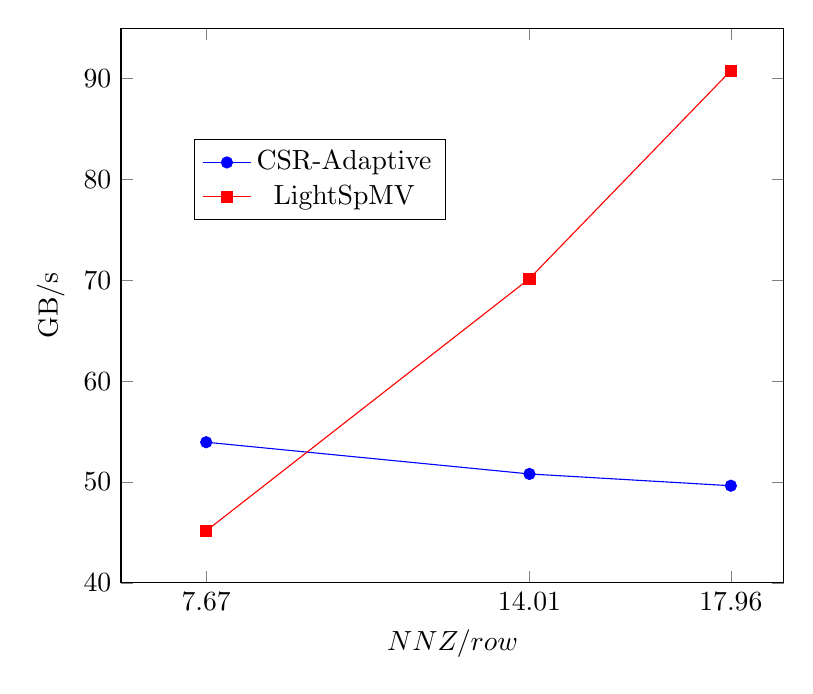
\begin{tikzpicture}
			\begin{axis}[        xlabel={$NNZ/row$},        ylabel={GB/s},        xmin=6, xmax=19,        ymin=40, ymax=95,        xtick={7.67,14.01,17.96},        legend style={at={(0.3,0.8)},anchor=north},        ]
				\addplot[color=blue,mark=*] coordinates {
					(7.67,53.944108)
					(14.01,50.797288)
					(17.96,49.628232)
				};
				\addlegendentry{CSR-Adaptive}
				
				\addplot[color=red,mark=square*] coordinates {
					(7.67,45.154160)
					(14.01,70.166256)
					(17.96,90.792728)
				};
				\addlegendentry{LightSpMV}
				
			\end{axis}
		\end{tikzpicture}
		\caption{GB/s vs. NNZ/row (Double precision).}
		\label{fig:my_label}
	\end{figure}
	
	
	
	
	
	
	
	
	
	
	
	
	
	\section{C Code Box or Inline}
	
	
	
	
	
	
	
	
	
	\section{Tables of Contents}
	
	
	
	
	
	
	
	
	
	
	\section{Reference}
	
	% to remove the hyperline rectangle
	
	\begin{lstlisting}[style=latexstyle]
		% to remove the hyperline rectangle
		\hypersetup{
			colorlinks=true,
			linkcolor=black,
			urlcolor=blue
		}
	\end{lstlisting}
	
	
	
	
	
	
	
	
	
	
	\textbf{linking a text file to a website, to a part of document, or mentioning an article as reference}
	
	
	
	
	\clearpage
	
\end{document}